\documentclass{standalone}
\usepackage{tikz}
\usetikzlibrary{patterns, positioning}
\usepackage[sfdefault]{ClearSans} %% option 'sfdefault' activates Clear Sans as the default text font
\usepackage[T1]{fontenc}

\begin{document}
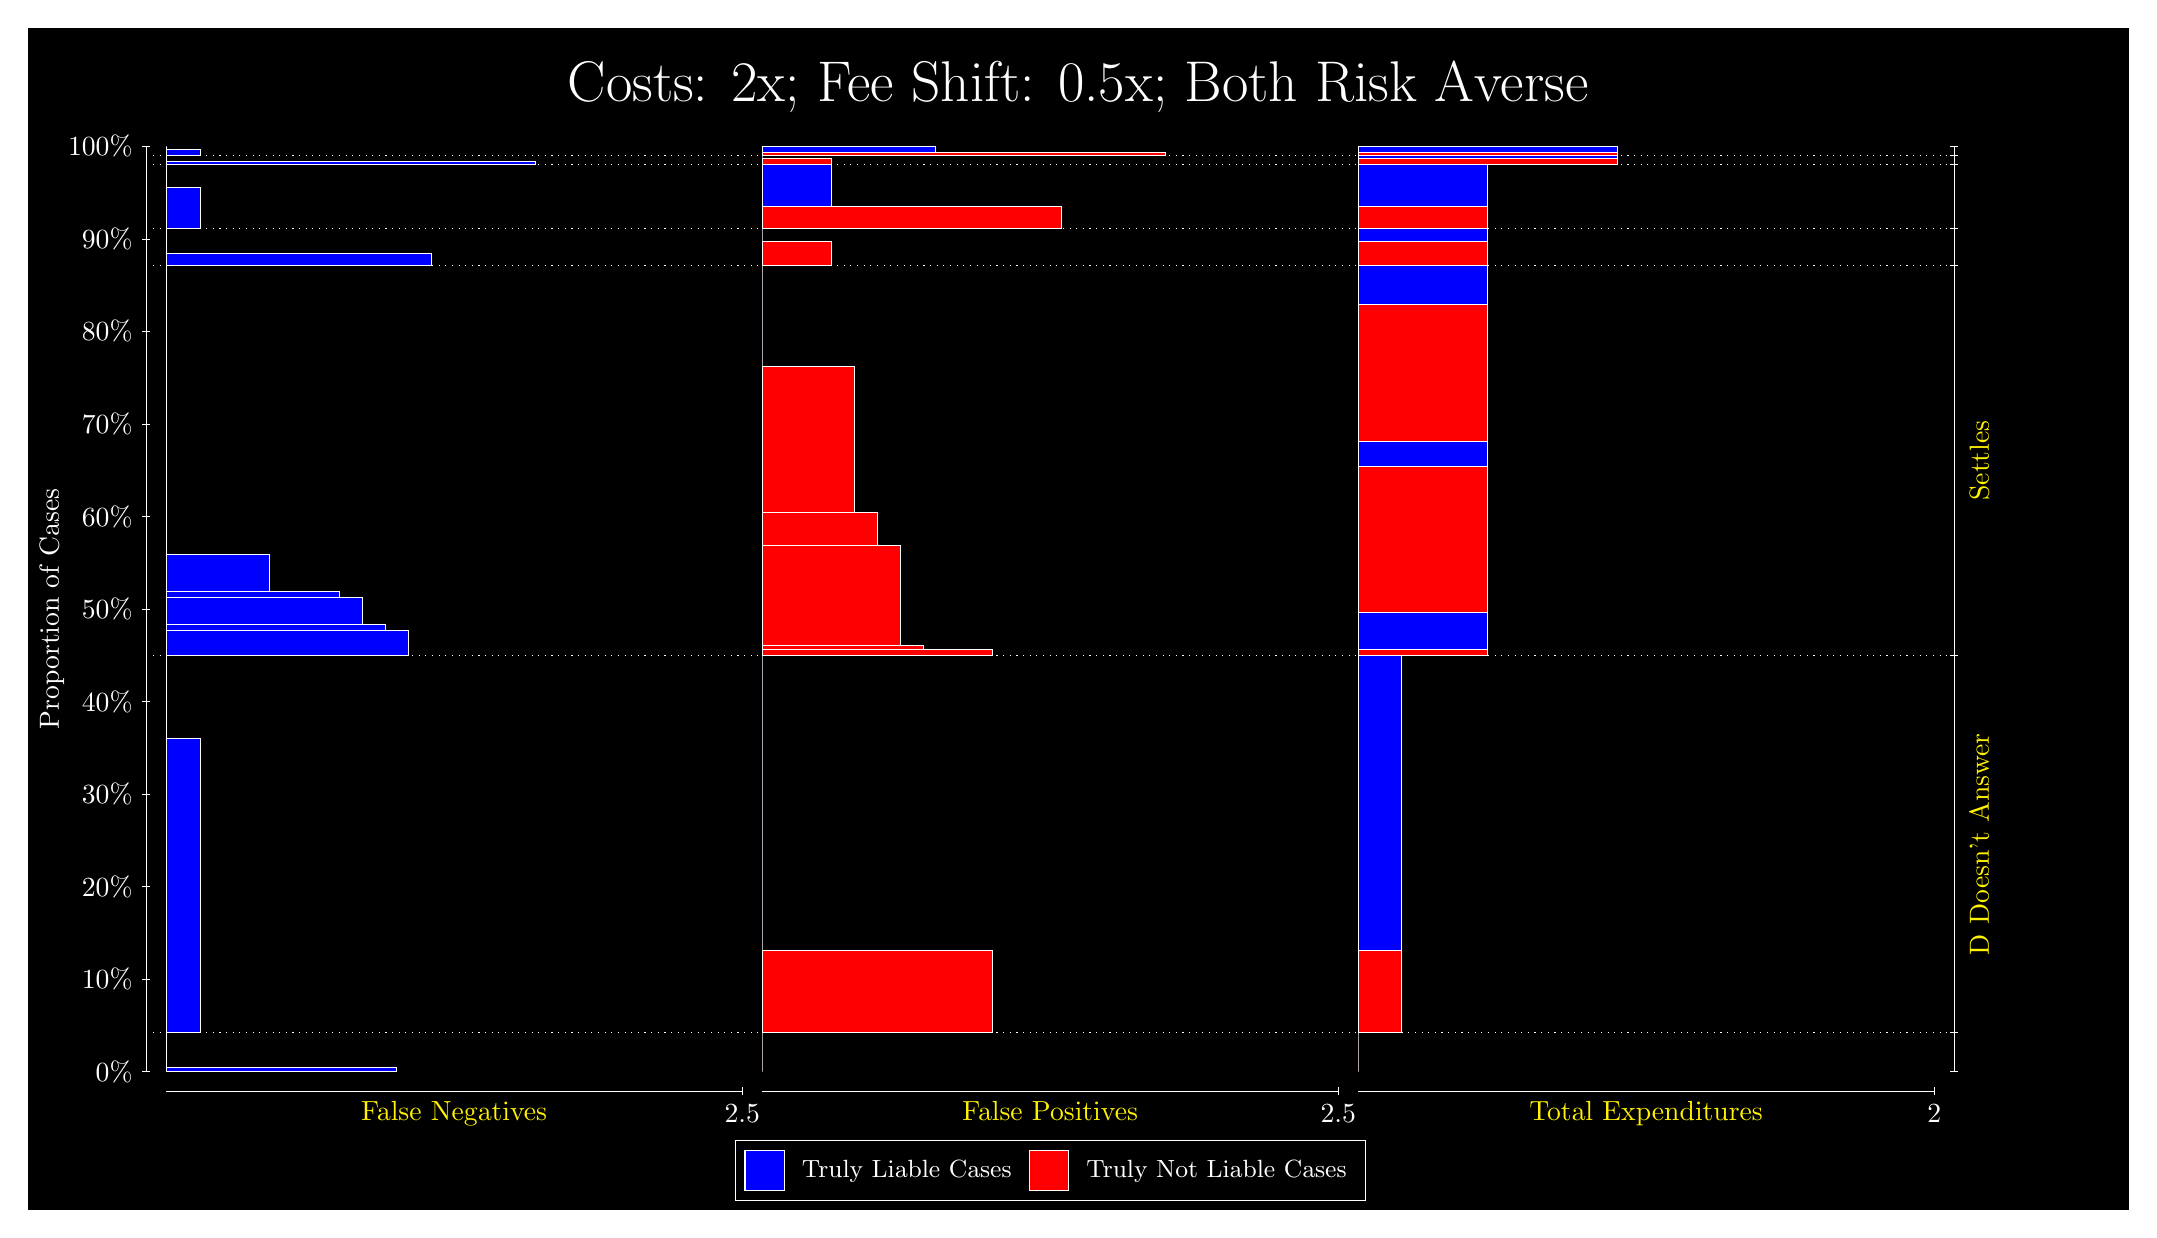
\begin{tikzpicture}
\draw[fill=black] (0,0) rectangle (26.667,15);
\draw[text=white] (0,13.5) rectangle (26.667,15) node[midway] {\huge Costs: 2x; Fee Shift: 0.5x; Both Risk Averse};
\draw[white, very thin] (1.5,1.75) -- (1.5,13.5);
\node[rotate=90, text=white, anchor=center] at (0.3, 7.625) {Proportion of Cases};
\draw[white, very thin] (1.45,1.75) -- (1.55,1.75);
\node[text=white, anchor=east] at (1.45, 1.75) {0\%};
\draw[white, very thin] (1.45,2.925) -- (1.55,2.925);
\node[text=white, anchor=east] at (1.45, 2.925) {10\%};
\draw[white, very thin] (1.45,4.1) -- (1.55,4.1);
\node[text=white, anchor=east] at (1.45, 4.1) {20\%};
\draw[white, very thin] (1.45,5.275) -- (1.55,5.275);
\node[text=white, anchor=east] at (1.45, 5.275) {30\%};
\draw[white, very thin] (1.45,6.45) -- (1.55,6.45);
\node[text=white, anchor=east] at (1.45, 6.45) {40\%};
\draw[white, very thin] (1.45,7.625) -- (1.55,7.625);
\node[text=white, anchor=east] at (1.45, 7.625) {50\%};
\draw[white, very thin] (1.45,8.8) -- (1.55,8.8);
\node[text=white, anchor=east] at (1.45, 8.8) {60\%};
\draw[white, very thin] (1.45,9.975) -- (1.55,9.975);
\node[text=white, anchor=east] at (1.45, 9.975) {70\%};
\draw[white, very thin] (1.45,11.15) -- (1.55,11.15);
\node[text=white, anchor=east] at (1.45, 11.15) {80\%};
\draw[white, very thin] (1.45,12.325) -- (1.55,12.325);
\node[text=white, anchor=east] at (1.45, 12.325) {90\%};
\draw[white, very thin] (1.45,13.5) -- (1.55,13.5);
\node[text=white, anchor=east] at (1.45, 13.5) {100\%};

\draw[white, very thin] (24.457,1.75) -- (24.457,13.5);
\draw[white, very thin] (24.407,1.75) -- (24.507,1.75);
\node[anchor=west] at (24.407, 1.75) {};
\draw[white, very thin] (24.407,2.2454) -- (24.507,2.2454);
\node[anchor=west] at (24.407, 2.2454) {};
\draw[white, very thin] (24.407,7.0308) -- (24.507,7.0308);
\node[anchor=west] at (24.407, 7.0308) {};
\draw[white, very thin] (24.407,11.991) -- (24.507,11.991);
\node[anchor=west] at (24.407, 11.991) {};
\draw[white, very thin] (24.407,12.454) -- (24.507,12.454);
\node[anchor=west] at (24.407, 12.454) {};
\draw[white, very thin] (24.407,13.267) -- (24.507,13.267);
\node[anchor=west] at (24.407, 13.267) {};
\draw[white, very thin] (24.407,13.389) -- (24.507,13.389);
\node[anchor=west] at (24.407, 13.389) {};
\draw[white, very thin] (24.407,13.5) -- (24.507,13.5);
\node[anchor=west] at (24.407, 13.5) {};

\draw[white, very thin, fill=blue] (1.75,1.75) rectangle (4.6775,1.8021);
\draw[white, very thin, fill=red] (1.75,1.8021) rectangle (1.75,2.2454);
\draw[white, very thin, fill=blue] (1.75,2.2454) rectangle (2.1891,5.9878);
\draw[white, very thin, fill=red] (1.75,5.9878) rectangle (1.75,7.0308);
\draw[white, very thin, fill=blue] (1.75,7.0308) rectangle (4.8239,7.3511);
\draw[white, very thin, fill=blue] (1.75,7.3511) rectangle (4.5312,7.433);
\draw[white, very thin, fill=blue] (1.75,7.433) rectangle (4.2384,7.779);
\draw[white, very thin, fill=blue] (1.75,7.779) rectangle (3.9457,7.8456);
\draw[white, very thin, fill=blue] (1.75,7.8456) rectangle (3.0674,8.3153);
\draw[white, very thin, fill=red] (1.75,8.3153) rectangle (1.75,11.991);
\draw[white, very thin, fill=blue] (1.75,11.991) rectangle (5.1167,12.147);
\draw[white, very thin, fill=red] (1.75,12.147) rectangle (1.75,12.454);
\draw[white, very thin, fill=blue] (1.75,12.454) rectangle (2.1891,12.983);
\draw[white, very thin, fill=red] (1.75,12.983) rectangle (1.75,13.267);
\draw[white, very thin, fill=blue] (1.75,13.267) rectangle (6.4341,13.304);
\draw[white, very thin, fill=red] (1.75,13.304) rectangle (1.75,13.389);
\draw[white, very thin, fill=blue] (1.75,13.389) rectangle (2.1891,13.462);
\draw[white, very thin, fill=red] (1.75,13.462) rectangle (1.75,13.5);
\draw[white, very thin, fill=red] (9.3189,1.75) rectangle (9.3189,2.1933);
\draw[white, very thin, fill=blue] (9.3189,2.1933) rectangle (9.3189,2.2454);
\draw[white, very thin, fill=red] (9.3189,2.2454) rectangle (12.246,3.2885);
\draw[white, very thin, fill=blue] (9.3189,3.2885) rectangle (9.3189,7.0308);
\draw[white, very thin, fill=red] (9.3189,7.0308) rectangle (12.246,7.115);
\draw[white, very thin, fill=red] (9.3189,7.115) rectangle (11.368,7.1686);
\draw[white, very thin, fill=red] (9.3189,7.1686) rectangle (11.075,8.4279);
\draw[white, very thin, fill=red] (9.3189,8.4279) rectangle (10.783,8.8524);
\draw[white, very thin, fill=red] (9.3189,8.8524) rectangle (10.49,10.707);
\draw[white, very thin, fill=blue] (9.3189,10.707) rectangle (9.3189,11.991);
\draw[white, very thin, fill=red] (9.3189,11.991) rectangle (10.197,12.298);
\draw[white, very thin, fill=blue] (9.3189,12.298) rectangle (9.3189,12.454);
\draw[white, very thin, fill=red] (9.3189,12.454) rectangle (13.125,12.738);
\draw[white, very thin, fill=blue] (9.3189,12.738) rectangle (10.197,13.267);
\draw[white, very thin, fill=red] (9.3189,13.267) rectangle (10.197,13.351);
\draw[white, very thin, fill=blue] (9.3189,13.351) rectangle (9.3189,13.389);
\draw[white, very thin, fill=red] (9.3189,13.389) rectangle (14.442,13.426);
\draw[white, very thin, fill=blue] (9.3189,13.426) rectangle (11.515,13.5);
\draw[white, very thin, fill=red] (16.888,1.75) rectangle (16.888,2.1933);
\draw[white, very thin, fill=blue] (16.888,2.1933) rectangle (16.888,2.2454);
\draw[white, very thin, fill=red] (16.888,2.2454) rectangle (17.437,3.2885);
\draw[white, very thin, fill=blue] (16.888,3.2885) rectangle (17.437,7.0308);
\draw[white, very thin, fill=red] (16.888,7.0308) rectangle (18.534,7.115);
\draw[white, very thin, fill=blue] (16.888,7.115) rectangle (18.534,7.5847);
\draw[white, very thin, fill=red] (16.888,7.5847) rectangle (18.534,9.4388);
\draw[white, very thin, fill=blue] (16.888,9.4388) rectangle (18.534,9.7591);
\draw[white, very thin, fill=red] (16.888,9.7591) rectangle (18.534,11.497);
\draw[white, very thin, fill=blue] (16.888,11.497) rectangle (18.534,11.991);
\draw[white, very thin, fill=red] (16.888,11.991) rectangle (18.534,12.298);
\draw[white, very thin, fill=blue] (16.888,12.298) rectangle (18.534,12.454);
\draw[white, very thin, fill=red] (16.888,12.454) rectangle (18.534,12.738);
\draw[white, very thin, fill=blue] (16.888,12.738) rectangle (18.534,13.267);
\draw[white, very thin, fill=red] (16.888,13.267) rectangle (20.181,13.351);
\draw[white, very thin, fill=blue] (16.888,13.351) rectangle (20.181,13.389);
\draw[white, very thin, fill=red] (16.888,13.389) rectangle (20.181,13.426);
\draw[white, very thin, fill=blue] (16.888,13.426) rectangle (20.181,13.5);
\draw[white, dotted] (1.5,2.2454) -- (24.457,2.2454);
\draw[white, dotted] (1.5,7.0308) -- (24.457,7.0308);
\draw[white, dotted] (1.5,11.991) -- (24.457,11.991);
\draw[white, dotted] (1.5,12.454) -- (24.457,12.454);
\draw[white, dotted] (1.5,13.267) -- (24.457,13.267);
\draw[white, dotted] (1.5,13.389) -- (24.457,13.389);
\draw[white, very thin] (1.75,1.5) -- (9.0689,1.5);
\node[text=yellow, anchor=north] at (5.4094, 1.5) {False Negatives};
\draw[white, very thin] (9.0689,1.45) -- (9.0689,1.55);
\node[text=white, anchor=north] at (9.0689, 1.45) {2.5};

\draw[white, very thin] (9.3189,1.5) -- (16.638,1.5);
\node[text=yellow, anchor=north] at (12.978, 1.5) {False Positives};
\draw[white, very thin] (16.638,1.45) -- (16.638,1.55);
\node[text=white, anchor=north] at (16.638, 1.45) {2.5};

\draw[white, very thin] (16.888,1.5) -- (24.207,1.5);
\node[text=yellow, anchor=north] at (20.547, 1.5) {Total Expenditures};
\draw[white, very thin] (24.207,1.45) -- (24.207,1.55);
\node[text=white, anchor=north] at (24.207, 1.45) {2};


\node[text=yellow, centered, rotate=90] at (24.777, 4.6381) {D Doesn't Answer};
\node[text=yellow, centered, rotate=90] at (24.777, 9.5109) {Settles};





\draw (12.978300999999998,1.5) node[draw=none] (baseCoordinate) {};
\begin{scope}[align=center]
        \matrix[scale=0.5, draw=white, below=0.5cm of baseCoordinate, nodes={draw}, column sep=0.1cm]{
            \node[rectangle, draw, minimum width=0.5cm, minimum height=0.5cm, fill=blue] {}; &
            \node[draw=none, font=\small, text=white] (B) {Truly Liable Cases}; &
            \node[rectangle, draw, minimum width=0.5cm, minimum height=0.5cm, fill=red] {}; &
            \node[draw=none, font=\small, text=white] (B) {Truly Not Liable Cases}; \\
            };
\end{scope}

\end{tikzpicture}
\end{document}